% file: PGO_5_2_sims_1.tex
% created by Orbiter tikz interface
% creation date: Mon Dec 21 16:40:00 MST 2020
% DeviceCoordinates 0 0 1000000 1000000
% UserCoordinates 0 0 10000 10000
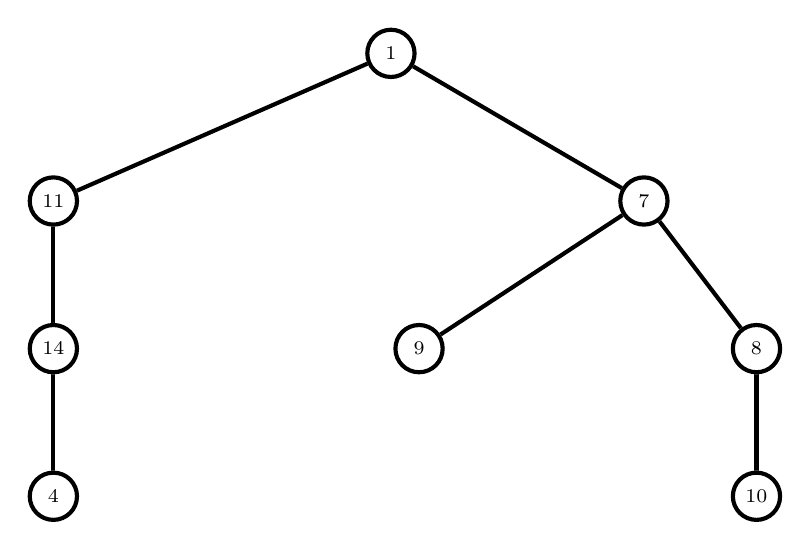
\begin{tikzpicture}[scale=0.45,line width = 1.5pt]
\draw [] (16.6667,31.25) -- (7.14,27.0833);
\draw [] (16.6667,31.25) -- (23.8067,27.0833);
\draw [] (7.14,27.0833) -- (7.14,22.9167);
\draw [] (23.8067,27.0833) -- (17.46,22.9167);
\draw [] (23.8067,27.0833) -- (26.9833,22.9167);
\draw [] (7.14,22.9167) -- (7.14,18.75);
\draw [] (26.9833,22.9167) -- (26.9833,18.75);
\filldraw[color=white] (16.6667,31.25) circle [radius = 0.666667cm];
\draw (16.6667,31.25) circle [radius = 0.666667cm];
\draw (16.6667,31.25) node{{\scriptsize 1}};
\filldraw[color=white] (7.14,27.0833) circle [radius = 0.666667cm];
\draw (7.14,27.0833) circle [radius = 0.666667cm];
\draw (7.14,27.0833) node{{\scriptsize 11}};
\filldraw[color=white] (23.8067,27.0833) circle [radius = 0.666667cm];
\draw (23.8067,27.0833) circle [radius = 0.666667cm];
\draw (23.8067,27.0833) node{{\scriptsize 7}};
\filldraw[color=white] (7.14,22.9167) circle [radius = 0.666667cm];
\draw (7.14,22.9167) circle [radius = 0.666667cm];
\draw (7.14,22.9167) node{{\scriptsize 14}};
\filldraw[color=white] (17.46,22.9167) circle [radius = 0.666667cm];
\draw (17.46,22.9167) circle [radius = 0.666667cm];
\draw (17.46,22.9167) node{{\scriptsize 9}};
\filldraw[color=white] (26.9833,22.9167) circle [radius = 0.666667cm];
\draw (26.9833,22.9167) circle [radius = 0.666667cm];
\draw (26.9833,22.9167) node{{\scriptsize 8}};
\filldraw[color=white] (7.14,18.75) circle [radius = 0.666667cm];
\draw (7.14,18.75) circle [radius = 0.666667cm];
\draw (7.14,18.75) node{{\scriptsize 4}};
\filldraw[color=white] (26.9833,18.75) circle [radius = 0.666667cm];
\draw (26.9833,18.75) circle [radius = 0.666667cm];
\draw (26.9833,18.75) node{{\scriptsize 10}};
\end{tikzpicture}
